%--------------------
% Look-up sheet
% -------------------

% For larger parentheses use
% ( \big( \Big( \bigg( \Bigg(

% How to reset equation counter
% \setcounter{equation}{0}


%--------------------
% Packages
% -------------------
\documentclass[11pt,a4paper]{article}
\usepackage[utf8x]{inputenc}
\usepackage[T1]{fontenc}
\usepackage{pdfpages} % Including .pdf pages
\usepackage{mathptmx} % Use Times Font

\usepackage[pdftex]{graphicx} % Required for including pictures
% \usepackage[pdftex,linkcolor=black,pdfborder={0 0 0}]{hyperref} % Format links for pdf
\usepackage{calc} % To reset the counter in the document after title page
\usepackage{enumitem} % Includes lists
\usepackage{csquotes} % Exercise as quotes
\usepackage{amsmath} % For using "equation*" 
\usepackage{nicefrac} % For in-line fractions

\setcounter{equation}{0}% How to reset equation counter

\frenchspacing % No double spacing between sentences
\linespread{1.2} % Set linespace
\usepackage[a4paper, lmargin=0.1666\paperwidth, rmargin=0.1666\paperwidth, tmargin=0.1111\paperheight, bmargin=0.1111\paperheight]{geometry} %margins
%\usepackage{parskip}

\usepackage[all]{nowidow} % Tries to remove widows
\usepackage[protrusion=true,expansion=true]{microtype} % Improves typography, load after fontpackage is selected



%-----------------------
% Set pdf information and add title, fill in the fields
%-----------------------
% \hypersetup{ 	
% pdfsubject = {Nano-Optics},
% pdftitle = {Assignment 2},
% pdfauthor = {Vlad Tkachuk}
% }

%-----------------------
% Begin document
%-----------------------
\begin{document} 

\section{Theory}

\subsection*{Exercise 1}


\begin{figure}[ht]
    \centering
    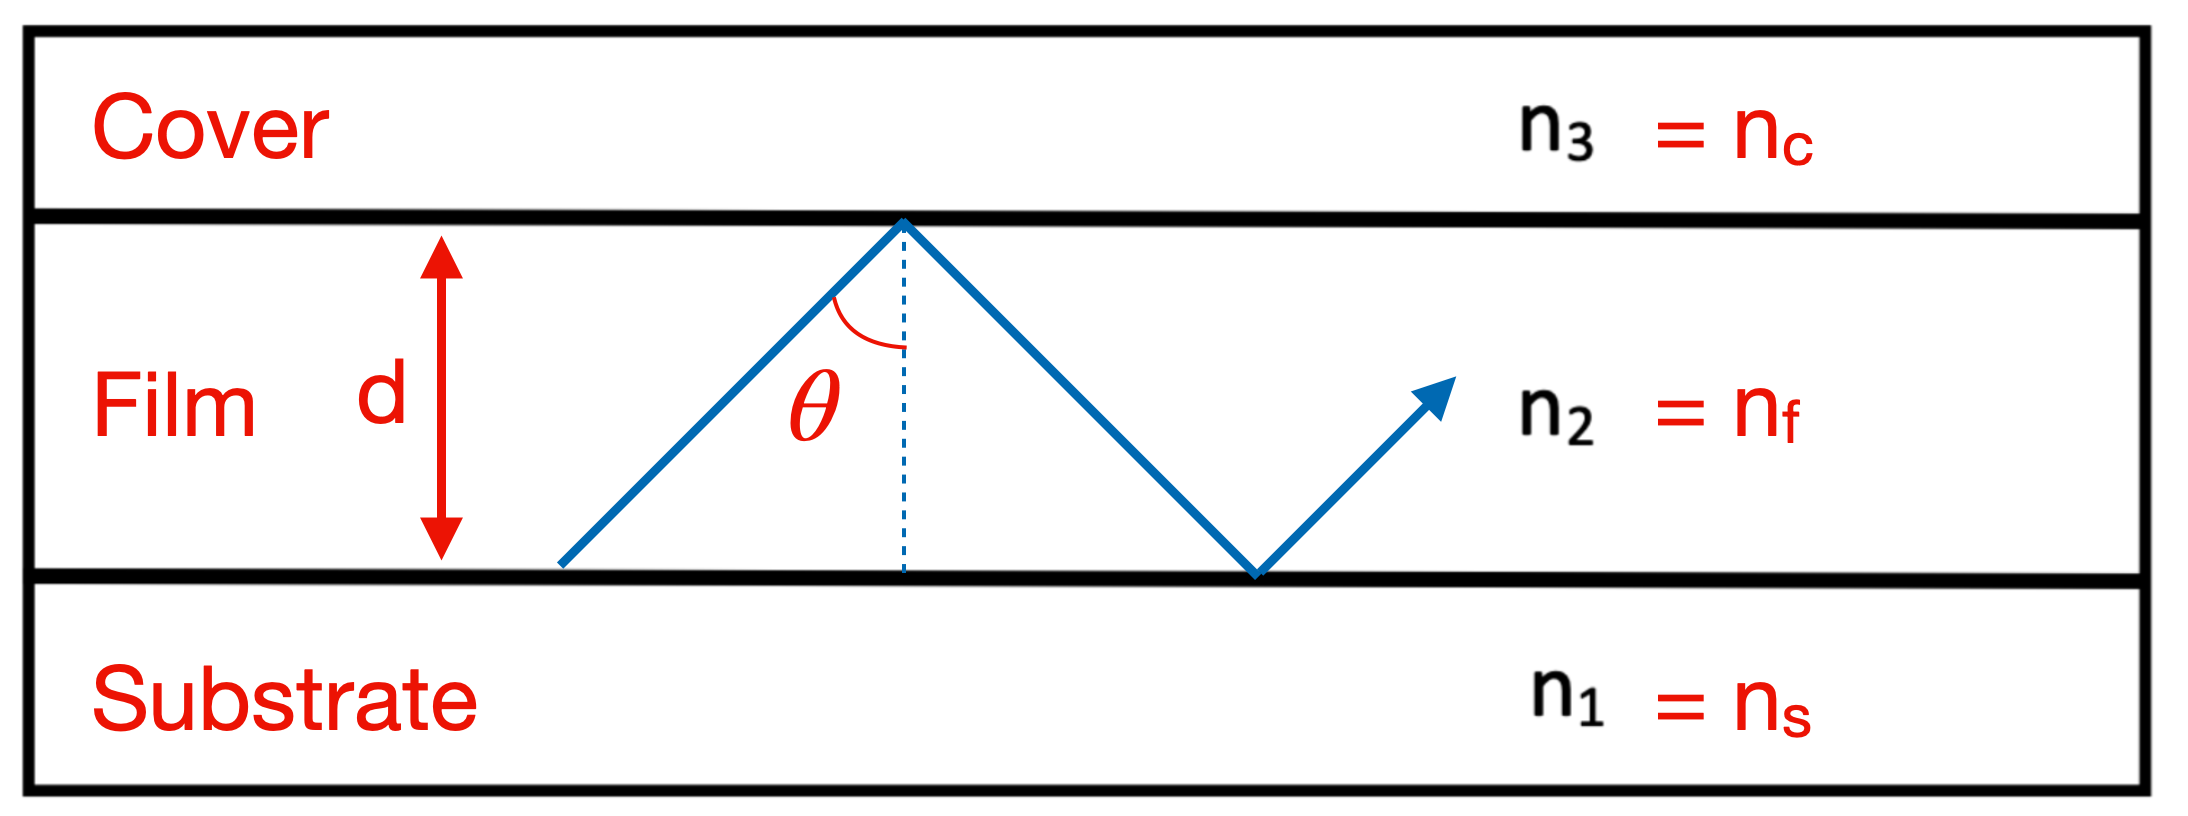
\includegraphics[width=0.5\textwidth]{fig_1.png}
    \caption{Schematic representation of a slab waveguide.}
\end{figure}


\begin{displayquote}
\textbf{(a)} Given the following waveguide refractive indices of the slab waveguide as 
depicted in Figure 1, $n_1=1.44$, $n_2=1$. 65, $n_3=1.33$, at a wavelength of 1.55 microns, 
calculate the minimum thickness for which there is a guided TE- mode. How can 
you reduce the thickness of the waveguide and still have a single guided mode? 
\end{displayquote}

Designate the layers as following on Figure 1. Start with the ray-optic approach 
self-consistency condition for total phase shift: 

\begin{equation}
    2k_{0} n_{f} d{} \cos{(\theta)}-\phi_{c} - \phi_{s} = 2 \pi{} m
\end{equation}

From (1), we can derive $d$:

\begin{equation}
    d = \frac{2\pi m + \phi_c + \phi_s}{2 k_0 n \cos{(\theta})}
\end{equation}

In our case, we are looking for zeroth order mode ($m=0$), because it corresponds to minimal waveguide thickness. $\theta=\max{(\theta_c,\theta_s)}$ represents the larger of total internal reflection angles: 
\begin{equation*}
    \theta_s=\arcsin{\Big(\frac{n_s}{n_f}}\Big)=1.061 \;[rad]   
\end{equation*}

\begin{equation*}
    \theta_c=\arcsin{\Big(\frac{n_c}{n_f}}\Big)=0.937 \;[rad]
\end{equation*}

By definition, 
\begin{equation}
    k_0=\frac{2\pi}{\lambda}=4.054\cdot{10^6} \; \bigg[\frac{1}{m}\bigg]
\end{equation}


The definition of reflection phase angle $\phi_{c,s}$ in (2) of the reflected TE waves:

\begin{equation}
    \tan{\Big(\frac{\phi_{s,c}}{2}\Big)}=\frac{\sqrt{{n_{f}}^2\sin^2{\theta}-{n_{s,c}}^2}}{n_f\cos{\theta}}  
\end{equation}

from which we obtain: 
\begin{equation}
\phi_{s,c}=2\arctan{\Bigg(\frac{\sqrt{{n_{f}}^2\sin^2{\theta}-{n_{s,c}}^2}}{n_f\cos{\theta}}\Bigg)} 
\end{equation}

from which we can calculate $\phi_s=0, \; \phi_c=1.202 \; [rad]$.

Collecting all terms together in (2) yields $d = 1.84\cdot{10^{-7}} \; [m]$.

\begin{displayquote}
    \textbf{(b)} What is the minimum thickness if the refractive indices are $n_1=1.44$, $n_2=3$, $n_3=1.44$? This is a symmetric waveguide. ($n_1=n_3$). Can you generalize the result that you obtained for this type of waveguides?
\end{displayquote}

In this case, $\phi_c=\phi_s=0$, so the zeroth order mode yields, from (2), $d=0$. The first order mode yields $2.945\cdot{10^{-7}} \; [m]$. 

The lowest-order mode of the symmetric waveguide does not exhibit a cutoff as all other modes do. In principle, any wavelength could be guided in this mode even with an incrementally small $n_f-n_c$. 


\begin{displayquote}
    \textbf{(c)} In the waveguide of (b), what kind of mode will have an effective refractive index of 1.33? And $n_{eff}=3.32$?
\end{displayquote}

Recall the definition of effective refractive index: $n_{eff}=n_f\sin{(\theta)}$. Hence we can analyze the angle, $\theta$, that would correspond to the given $n_{eff}$. For $n_{eff}=1.33, \; \theta = 0.459 \; [rad]$. This is lower than critical angle, $0.501 \; [rad]$, hence the mode will be radiated into the cladding. $n_{eff}=3.32, \; \theta$ is complex, hence propagation is impossible. 

\setcounter{equation}{0}
\subsection*{Exercise 2}

For the following assignments we will be considering a slab waveguide structure consisting of a 220 nm silicon core (n=3.47) and a SiO\textsubscript{2} cladding (n=1.45) at a design wavelength of 1550 nm.


For a slab waveguide analytical expression of the field can be found by solving the wave equation using separation of variables. This leaves us with an eigenvalue problem to find the allowed modes of the waveguide.

\begin{displayquote}
   \textbf{(a)} Graphically or numerically solve the eigenvalue equation for the slab waveguide TE modes and obtain the effective refractive index $\beta_m=n_{eff}k_0$. Give a Plot of the graphical solution and or attach your script and explain what it does. 
\end{displayquote}

Mathcad Prime 8 was used for the solution. Eigenvalue equation for a symmetric slab waveguide that we are looking for to solve is: 

\begin{equation}
    \tan{dq}=\frac{2qp}{q^2-p^2}
\end{equation}

where we can express terms $p, \; q$ appearing in (1) as functions of $n_{eff}$:
\begin{equation*}
    p(n_{eff})=k_0\sqrt{n_{eff}^2-n_c^2}
\end{equation*}

\begin{equation*}
    q(n_{eff})=k_0\sqrt{n_{f}^2-n_{eff}^2}
\end{equation*}
This gives us left and right sides of the equation as functions of $n_{eff}$, which we can plot to have an initial guess for the numeric solution:
\begin{equation*}
    left(n_{eff})=\tan{(d\cdot{p(n_{eff}))}}
\end{equation*}
\begin{equation*}
    right(n_{eff})=\frac{2q(n_{eff})\cdot{p(n_{eff})}}{q(n_{eff})^2-p(n_{eff})^2}
\end{equation*}


\begin{figure}[ht]
    \centering
    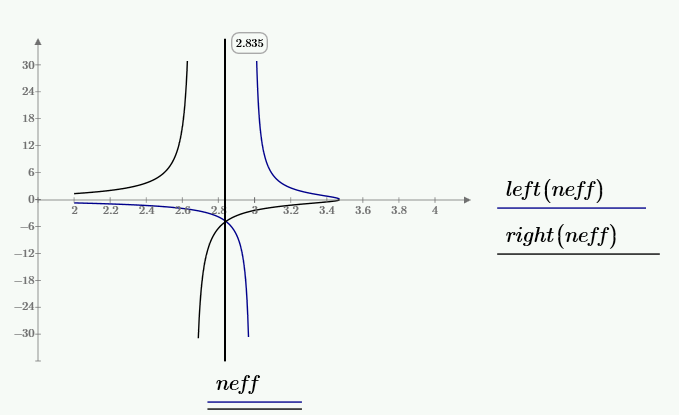
\includegraphics[width=0.75\textwidth]{fig_2.png}
    \caption{Graphical solution of the eigenvalue equation for the slab waveguide TE modes. The vertical marker is set manually.}
\end{figure}

Using the initial guess value of $n_{eff}=2.8$ we can then solve the equation numerically to obtain the required precision: $n_{eff}=2.842432$. The script is listed in Appendix. \\ \par

Due to the small size and high refractive index contrast between the core and cladding of the waveguide, coupling the light into it is difficult for two major reasons. The first is the alignment accuracy needed to overlap the input light with the waveguide mode. The second reason is that the mode of the input is hard to match to the mode of the waveguide, limiting the coupling efficiency. Calculating the efficiency is done by performing an overlap integral of the waveguide mode and incident mode.
For instance a standard 1550 nm fiber that can be connected to most other equipment in the lab, has a core diameter of 9 micrometer leading to a mode that is much larger than the waveguide mode. This severely limits the coupling efficiency. For this reason a grating coupler is often used to couple light into waveguides on integrated optical chips, as it allows for much better alignment tolerances and higher coupling efficiency for a standard 9 micron core fiber. In the following questions you will design a grating coupler for the waveguide of the exercise 2a. A schematic of a cross section of an integrated optical chip with a grating coupler is given in Figure 3.

\begin{displayquote}
    \textbf{(b)} Show that the period of a grating coupler is given by

    \begin{equation*}
        \Lambda=\frac{m2\pi}{k_0(n_{eff}-n_i\sin{(\theta_i)})}
    \end{equation*}
     where $\Lambda$ is the grating period, $m$ is the diffraction order that can take the values $m \; = \; 0, \; \pm1, \; \pm2 , \; ...$ and the incident $k$ is the cladding refractive index times the propagation constant in vacuum.
    Make a drawing of the grating coupler and indicate the involved $k$ vectors. Also give the phase matching condition for coupling into the waveguide mode.
    Hint: The angles are defined with respect to the normal, note that clockwise with respect to the normal is positive.
\end{displayquote}

The diffraction behavior for a grating coupler can be described using Bragg phase matching condition:
\begin{equation}
    \textbf{k}_0 n_i \sin{(\theta_i)} + m \textbf{G} = \beta_m
\end{equation}
where $\textbf{G}$ is grating vector, $\textbf{G}=\nicefrac{2\pi}{\Lambda}$ and $m$ is grating diffraction order. In order to preserve sign convention, we have to rearrange incoming light wave-vector (Figure 3). Using the fact that $\beta_m = n_{eff} k_0$, we can rearrange (2):

\begin{equation}
    \Lambda = \frac{2\pi m}{k_0 (n_{eff}-n_i \sin{(\theta_i)})}
\end{equation}

\begin{figure}[ht]
    \centering
    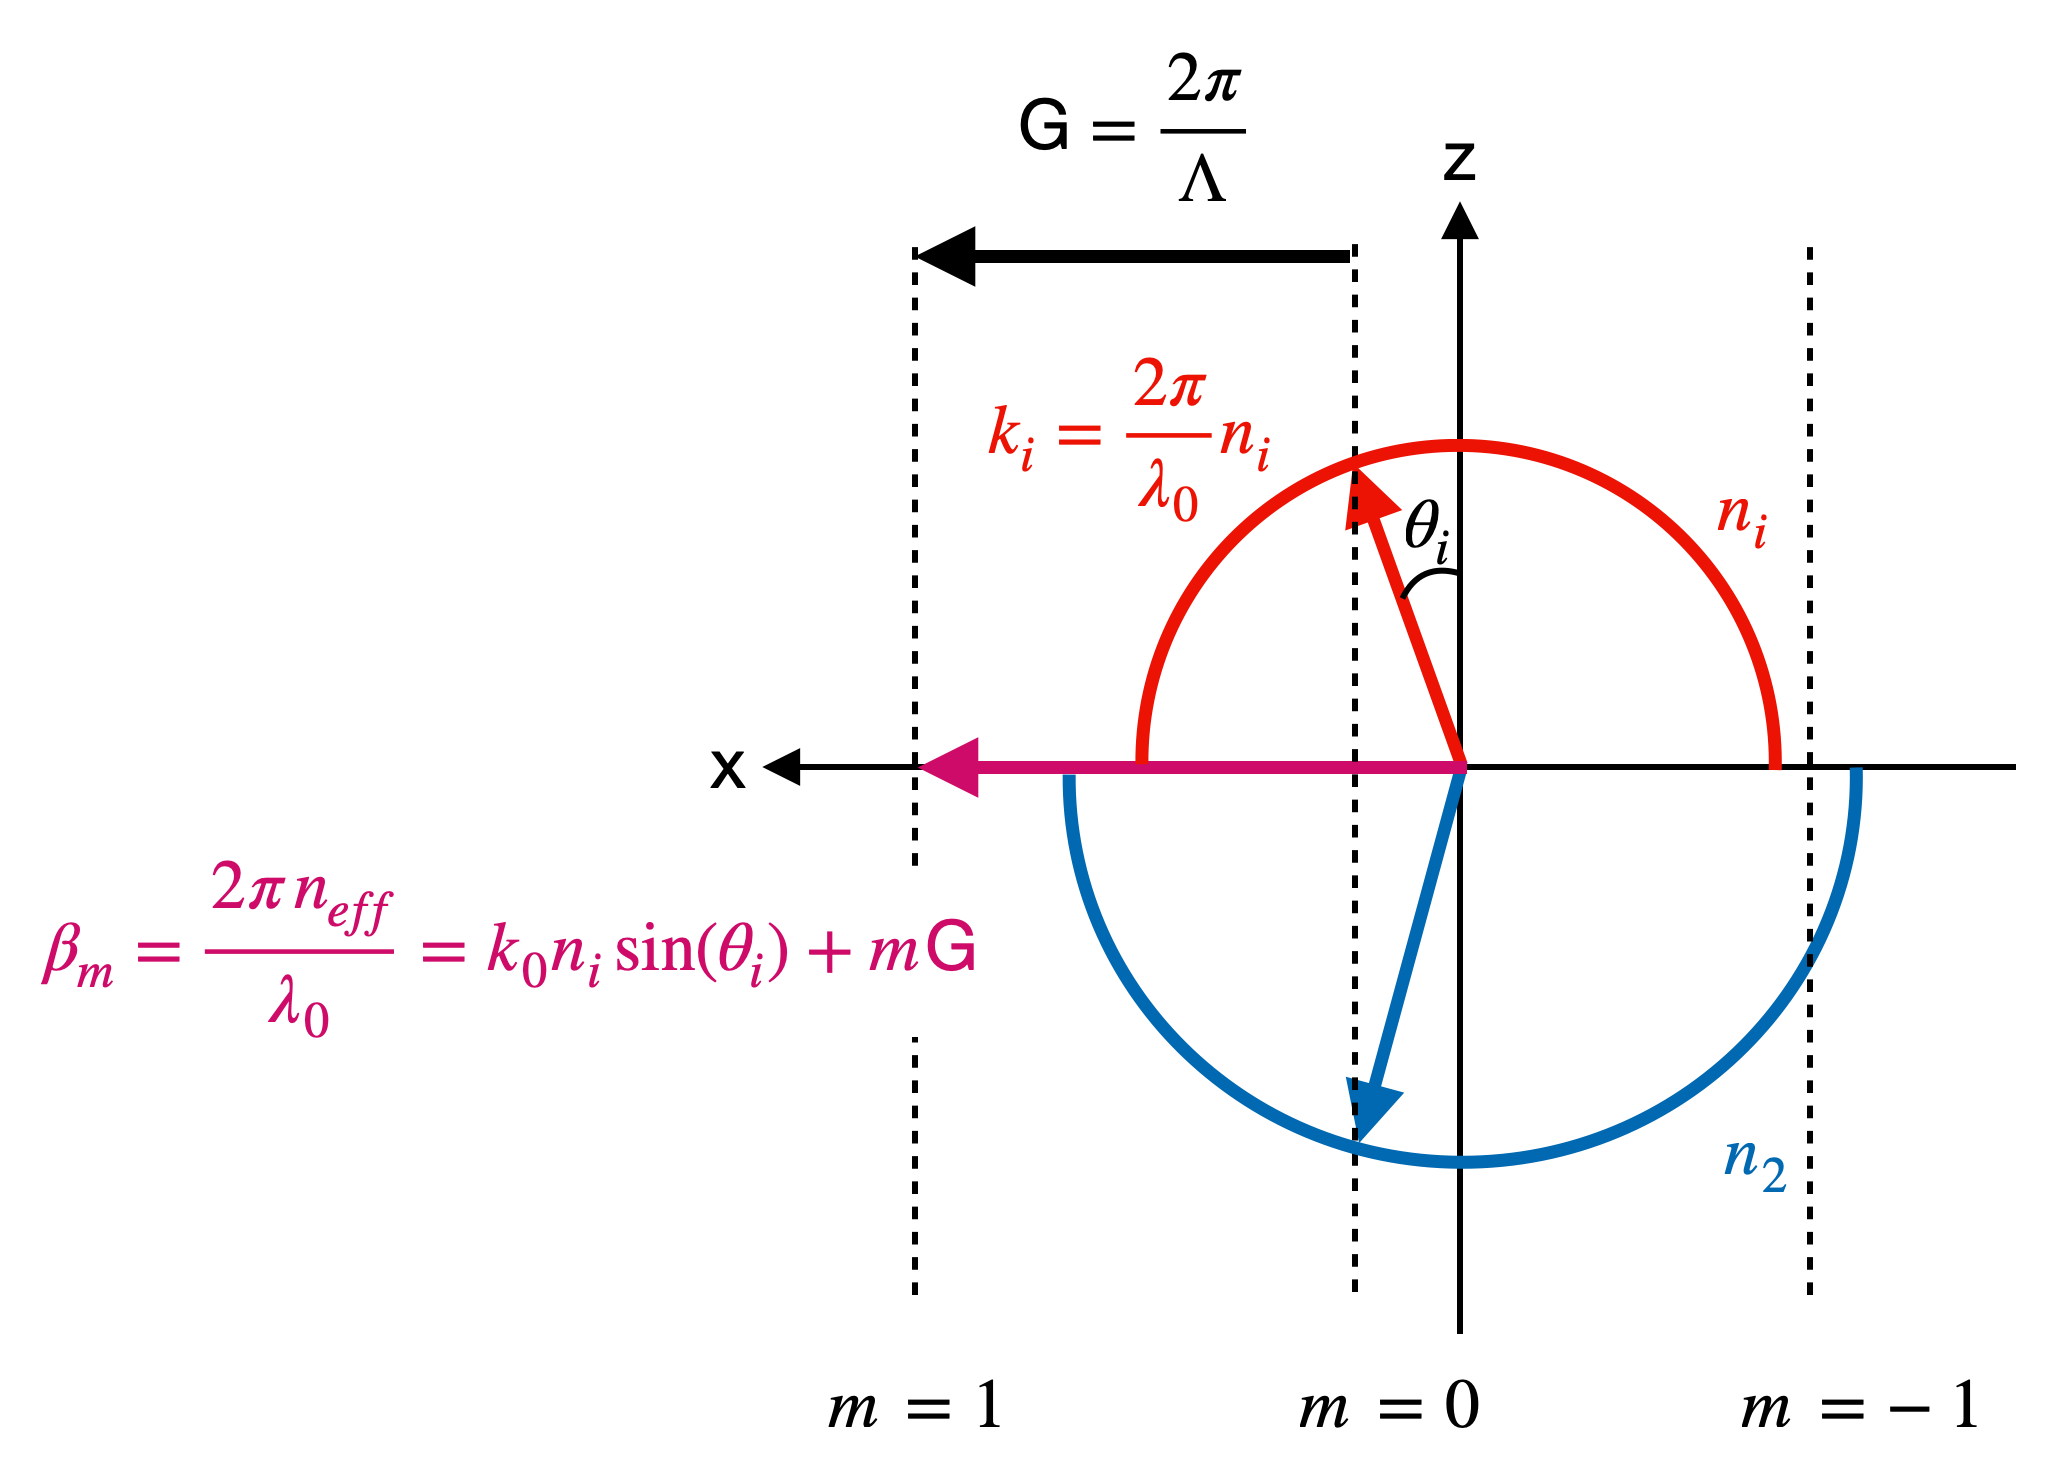
\includegraphics[width=0.75\textwidth]{fig_3.png}
    \caption{Wave-vector diagram for grating coupling.}
\end{figure}

\begin{displayquote}
    \textbf{(c)} Calculate the first order grating period for the waveguide of exercise 2a with the incident light from a fiber under an angle of 10 degrees with respect to the normal of the chips cladding surface. The fiber is suspended 10 micrometer above the silicon dioxide cladding layer. The fiber end facet is not cleaved under
an angle. Hint: make a drawing of the configuration. Note that $k_{in}=\nicefrac{2\pi}{\lambda_0}$.
\end{displayquote}

\begin{figure}[ht]
    \centering
    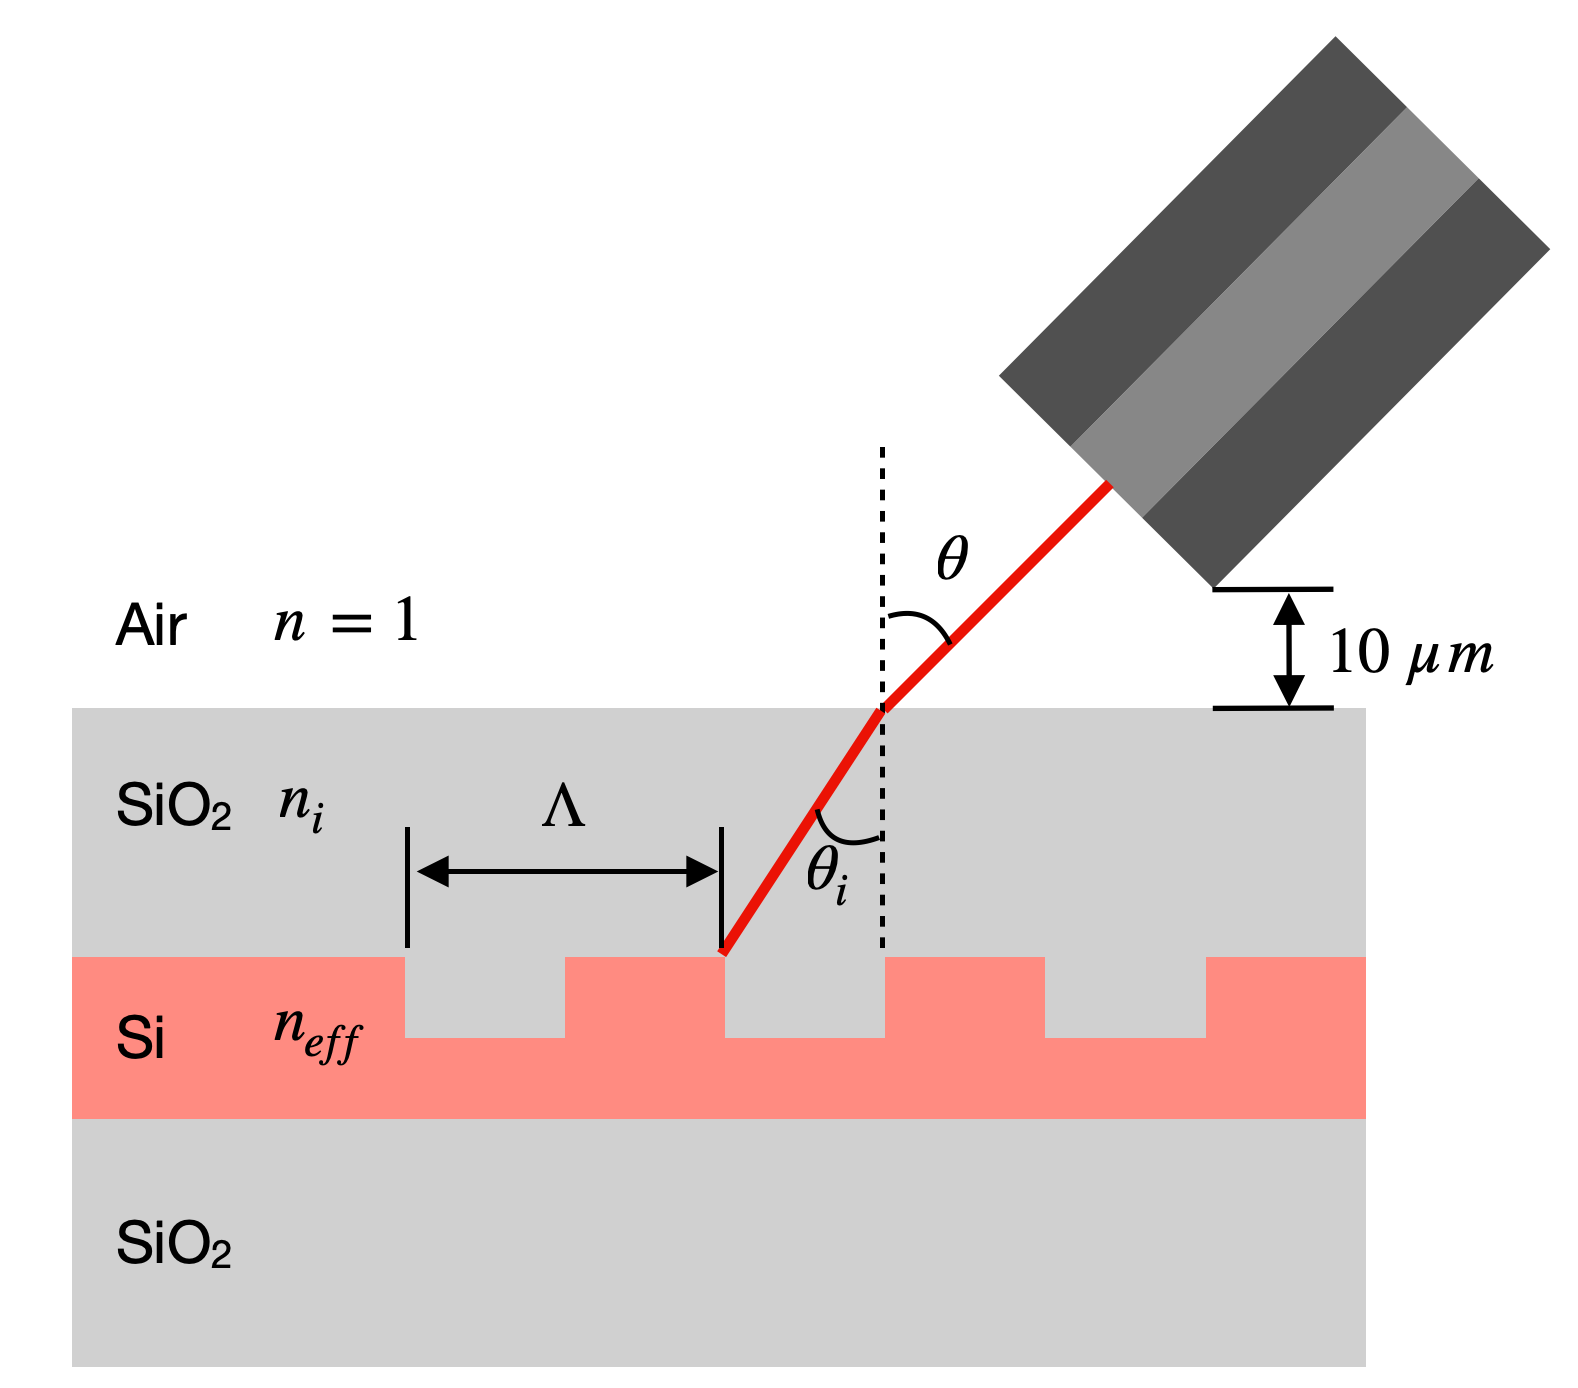
\includegraphics[width=0.5\textwidth]{fig_4.png}
    \caption{Schematic diagram of fiber-chip coupling.}
\end{figure}

The setup is schematically represented in Figure 4. The angle of incidence as observed by the grating is:

\begin{equation*}
    \sin{(\theta_i)}=\frac{\sin{(\theta)}}{n_{i}}
\end{equation*}

Hence by substituting all values in (3), we obtain:

\begin{equation*}
    \Lambda = \frac{2\pi}{\frac{2\pi}{1550\cdot{10^{-9}}}\cdot\Big(2.842432-1.45\cdot\frac{\sin{(0.175)}}{1.45}\Big)}=5.809\cdot10^{-7} \; [m]\approx580 \; [nm]
\end{equation*}

\newpage
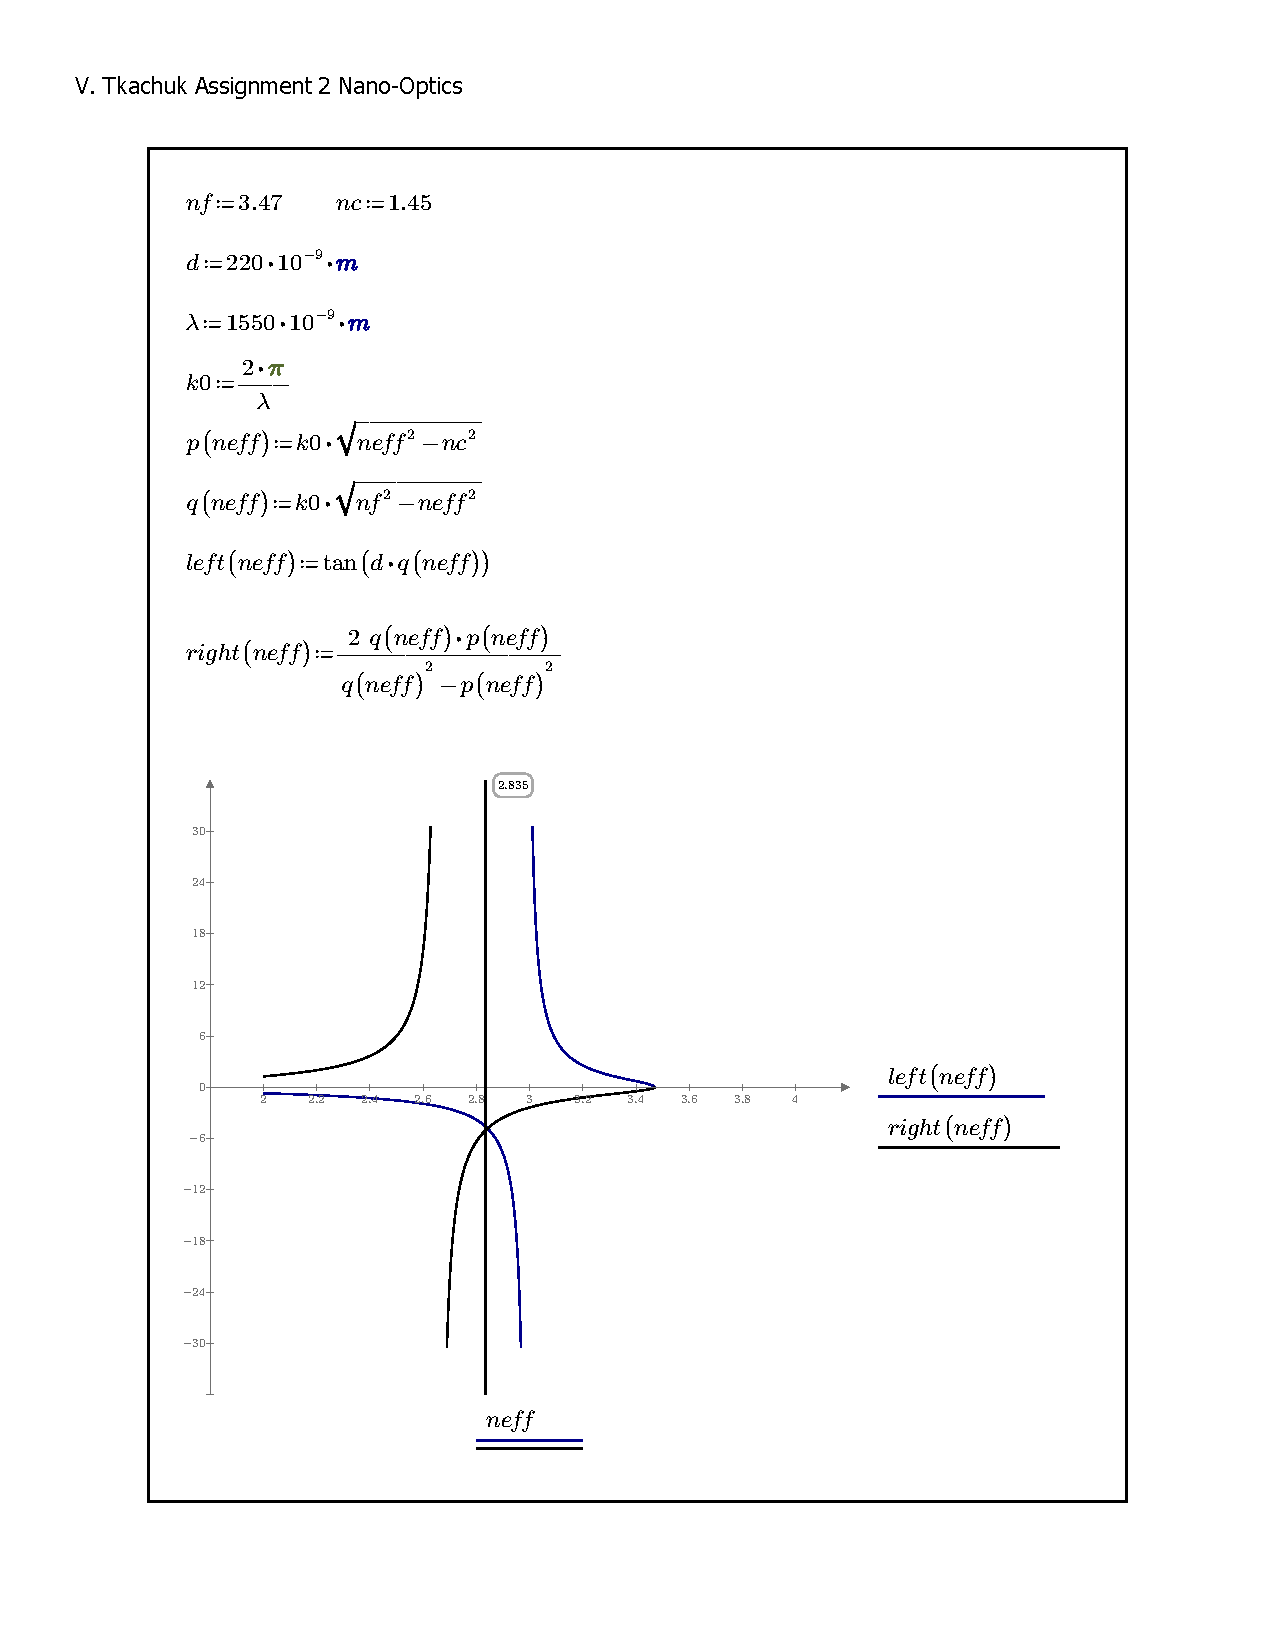
\includepdf[page=-]{app.pdf}

\section{Lumerical}

\subsection*{Exercise 1}

\begin{figure}[ht]
        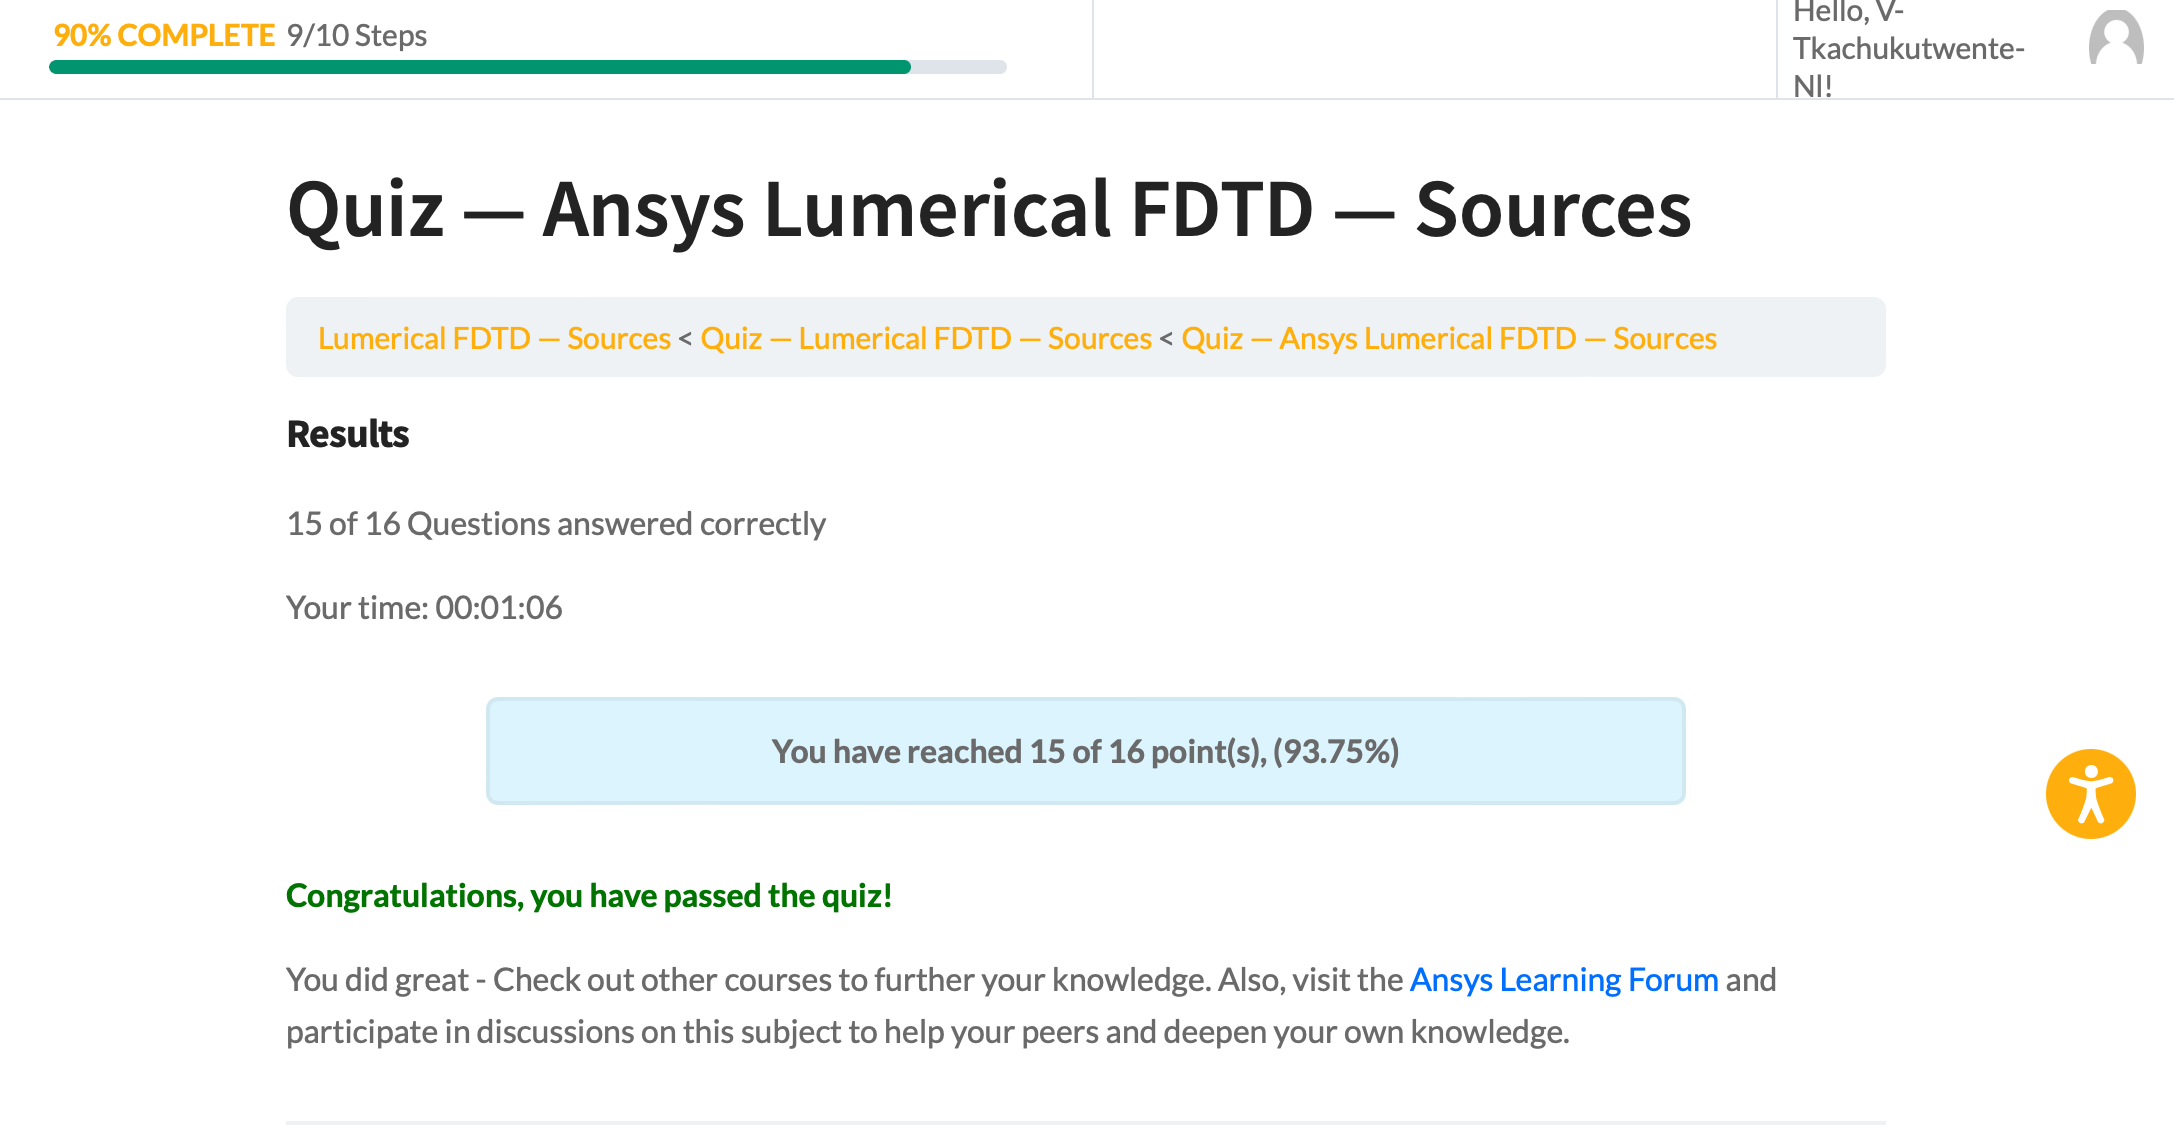
\includegraphics[width=0.95\textwidth]{lu1.png}
\end{figure}

\begin{figure}[ht]
        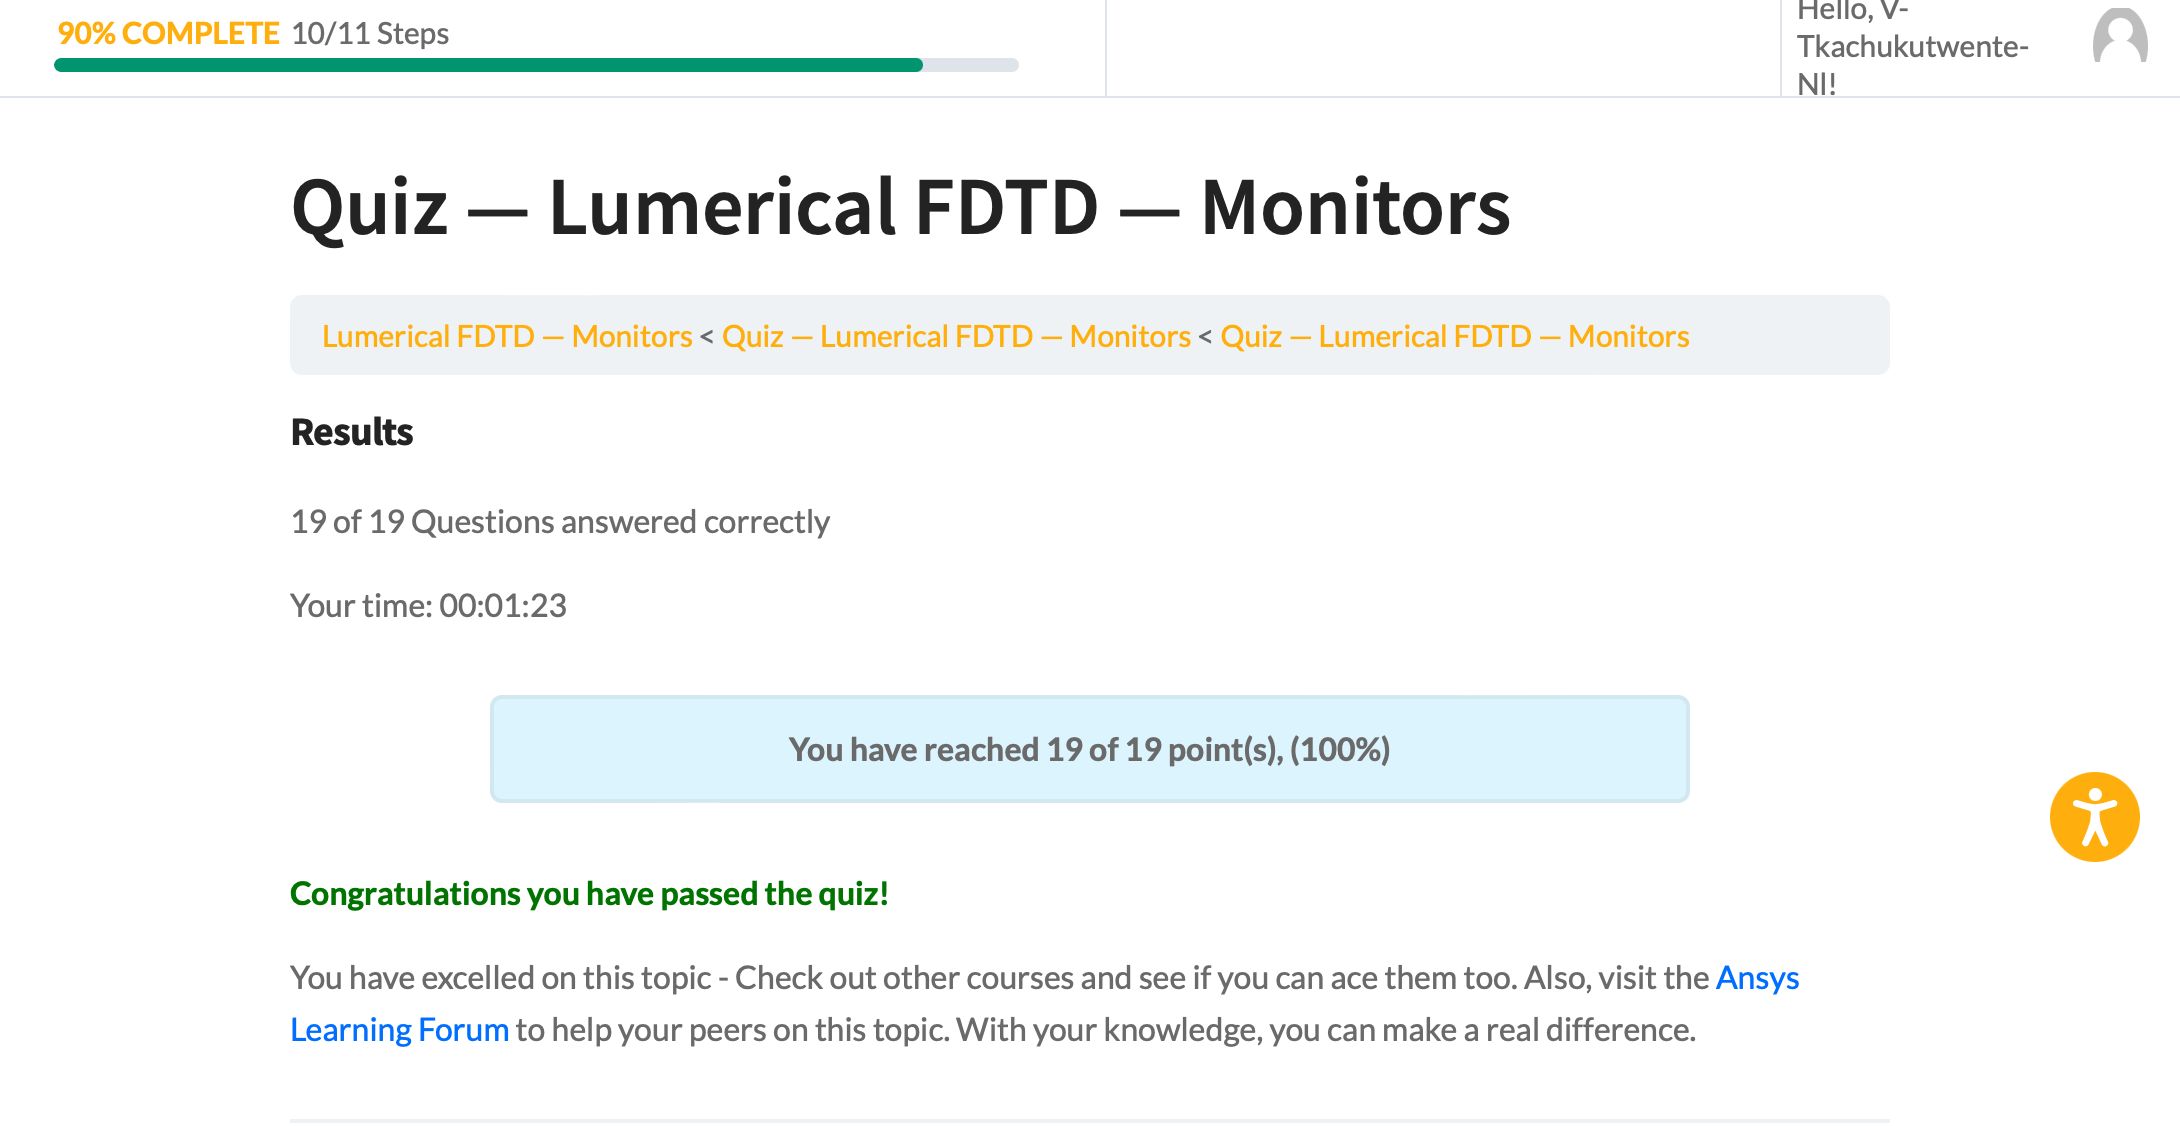
\includegraphics[width=0.95\textwidth]{lu2.png}
\end{figure}

\subsection*{Exercise 2}
\begin{displayquote}
    \textbf{1. }Which symmetries and the corresponding boundary conditions can be used to speed up the simulation? Apply the symmetry boundary conditions and show you get the same result.
\end{displayquote}

The geometry of the structure displays two-fold symmetry about the origin. The computation process can be sped up by applying\textit{ Anti-Symmetric} boundary condition at \textbf{x min bc}, and \textit{Symmetric} at \textbf{y min bc}. 

The results can be seen on Figures 5-9 below. While the computation time is four times less, some difference can be seen with the bump present. It is hence a trade-off to be considered, depending on the required precision of the simulation. 

\begin{displayquote}
    \textbf{2. } What happens when the polarization of the incident beam is rotated by 90 degrees? (note: switch off symmetry boundary conditions for this simulation at first) Does this change the correct symmetry boundary conditions? If yes change them and show you get the same result.
\end{displayquote}

Because the size of the structure is on the order of wavelength, rotating the polarization by 90 degrees affects the results quite strongly. Applying boundary conditions according to the polarization convention, thus \textit{Symmetric} boundary condition at \textbf{x min bc}, and \textit{Anti-Symmetric} at \textbf{y min bc}, affects the result even more dramatically. 

\begin{displayquote}
    \textbf{1.} Change the wavelength of the source to 405 nm, and set the correct beam options for a diffraction limited spot at the DVD surface for an objective of NA=0.85. ( use the scalar approximation) in the tab as indicated below.
\end{displayquote}

We have a selection of beam parameters to set. Let us use the angle and beam size: 
\begin{equation*}
    NA=n\sin{\theta} \; \Rightarrow \; \theta=\arcsin{\bigg(\frac{NA}{n}\bigg)}=33.26\deg
\end{equation*}

\begin{equation*}
    w_f=\frac{2\lambda}{\pi NA}= 303 \; [nm]
\end{equation*}

The original sweep gives optimal width of 200 nm for original beam parameters and wavelength. Tuning the source to the aforementioned parameters and wavelength, and sweeping again for the width between 10 nm and 100 nm in 6 steps, we obtain minimal signal between 28 and 64 nm (Figure 10). Running the length sweep from 100 nm to 600 nm in 6 steps, we obtain minimal signal for 140 nm (Figure 11). This is on the order of magnitude for the actual Blu-ray disc bumps, which are $150\times 130$ nm, and the spot size of 480 nm. Obviously, the real numbers are larger than those at the diffraction limit, as this provides margins for better reliability. 

We can now change the \textit{bumpwidth} and \textit{bumplength} to the found values in the script and run it to obtain the near- and far-field pictures (Figure 12, 13). It is evident that now the maxima of power distribution are dislocated not as far from each other as for the previous case with DVD, characterized by longer wavelength and geometric size of the bump. 

\begin{figure}
        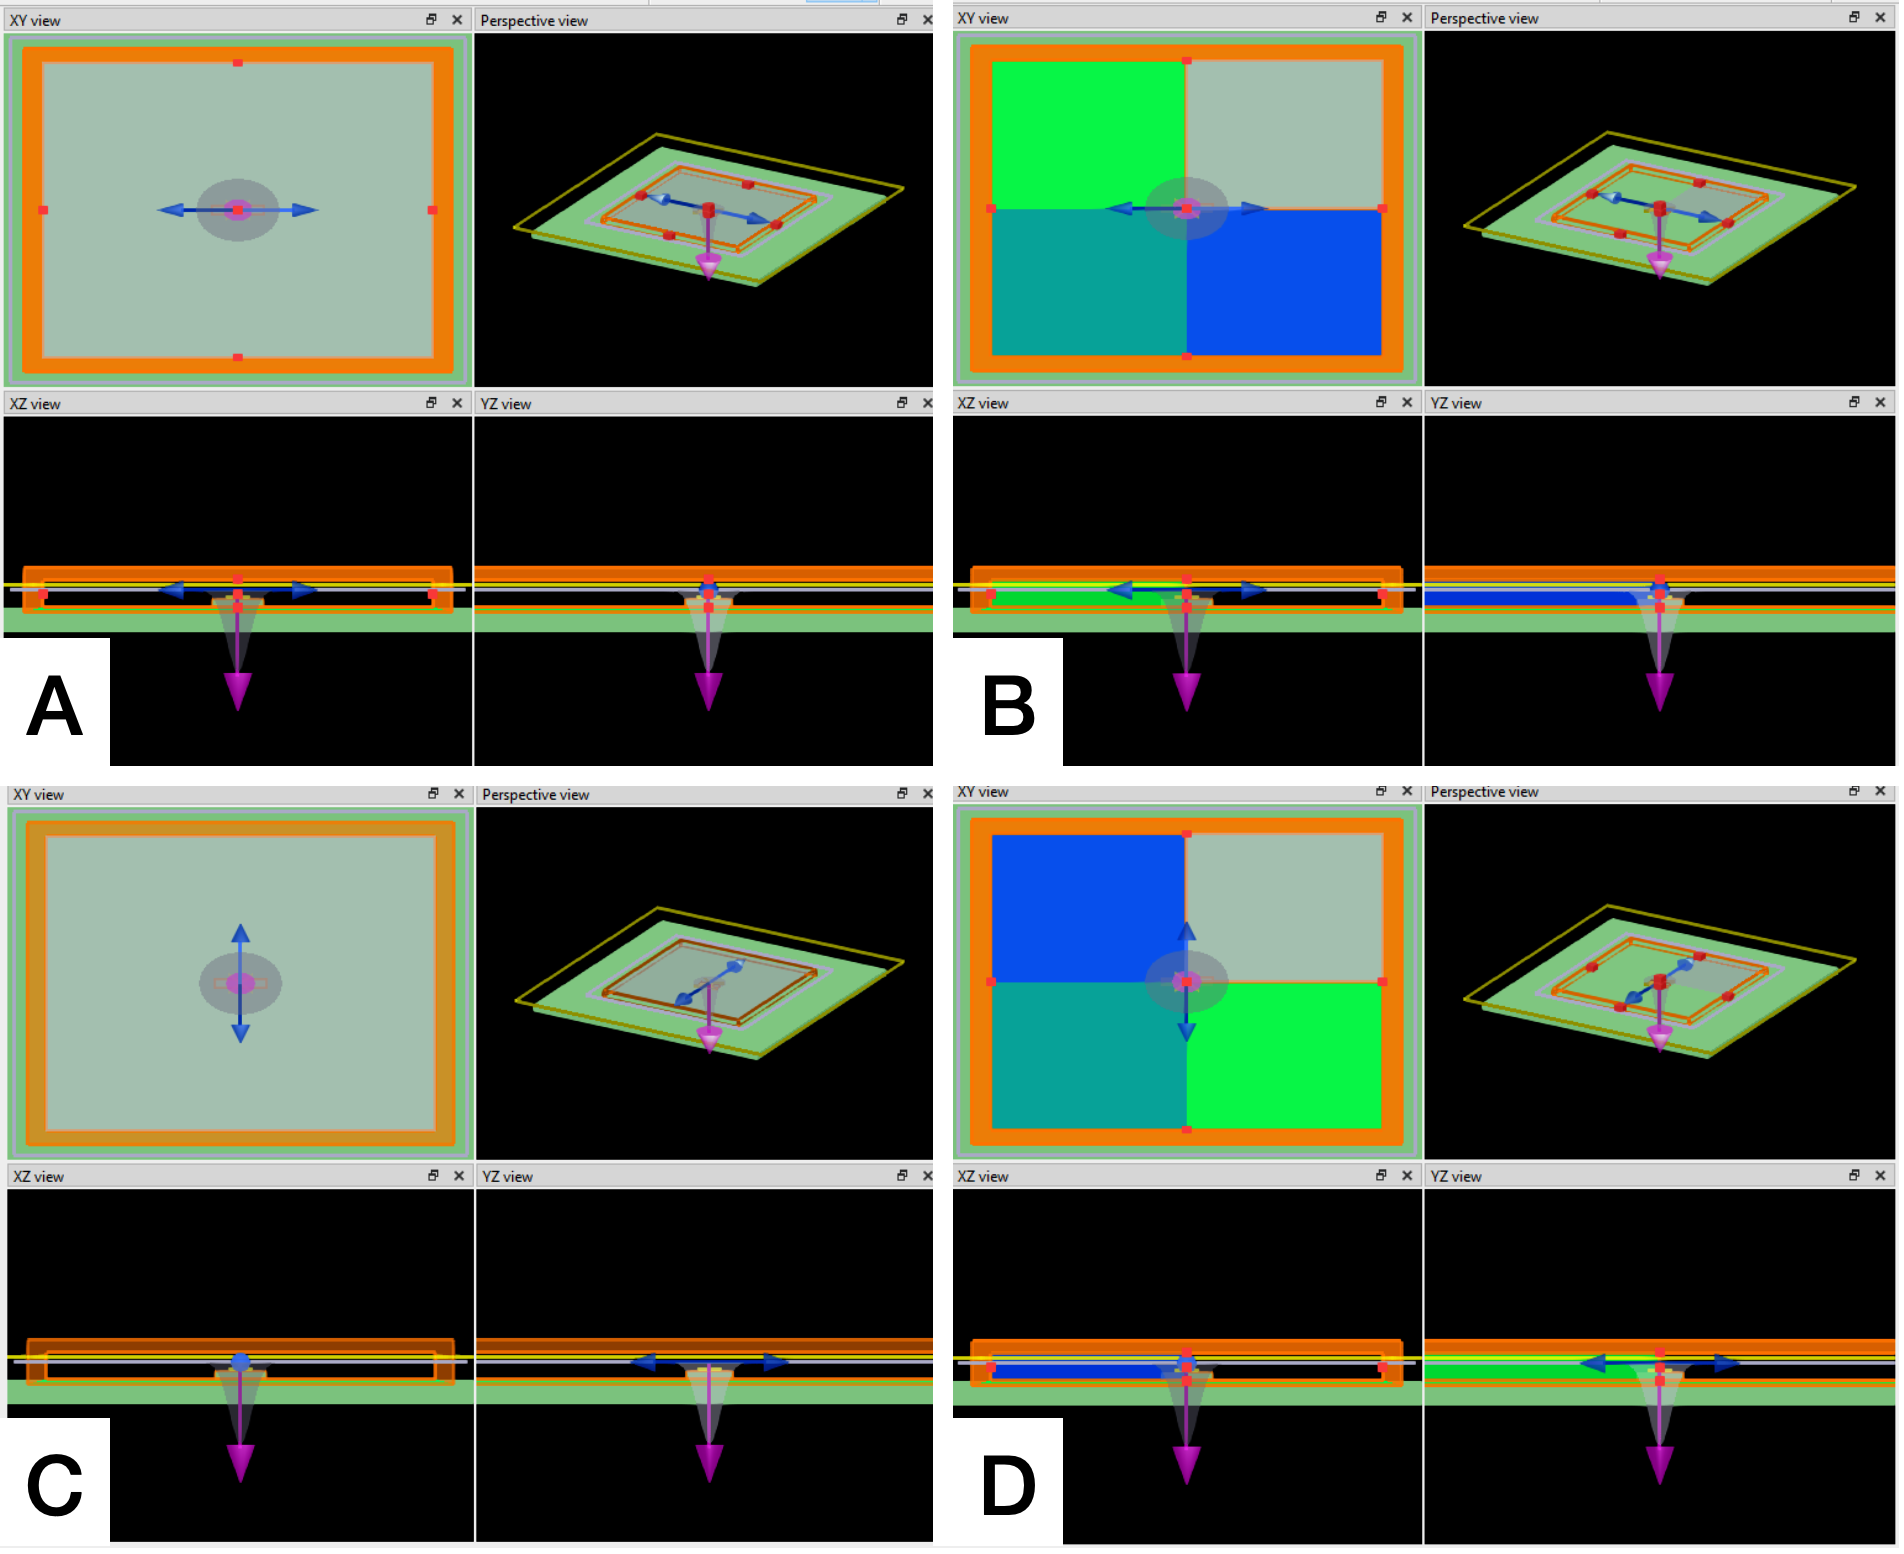
\includegraphics[width=0.95\textwidth]{1.png}
        \caption{Layout of the simulation. A - $0\deg$ polarization simulation. B - $0\deg$ polarization simulation, with boundary conditions applied. C - $90\deg$ polarization simulation. D - $90\deg$ polarization simulation, with boundary conditions applied.}
\end{figure}
\begin{figure}
        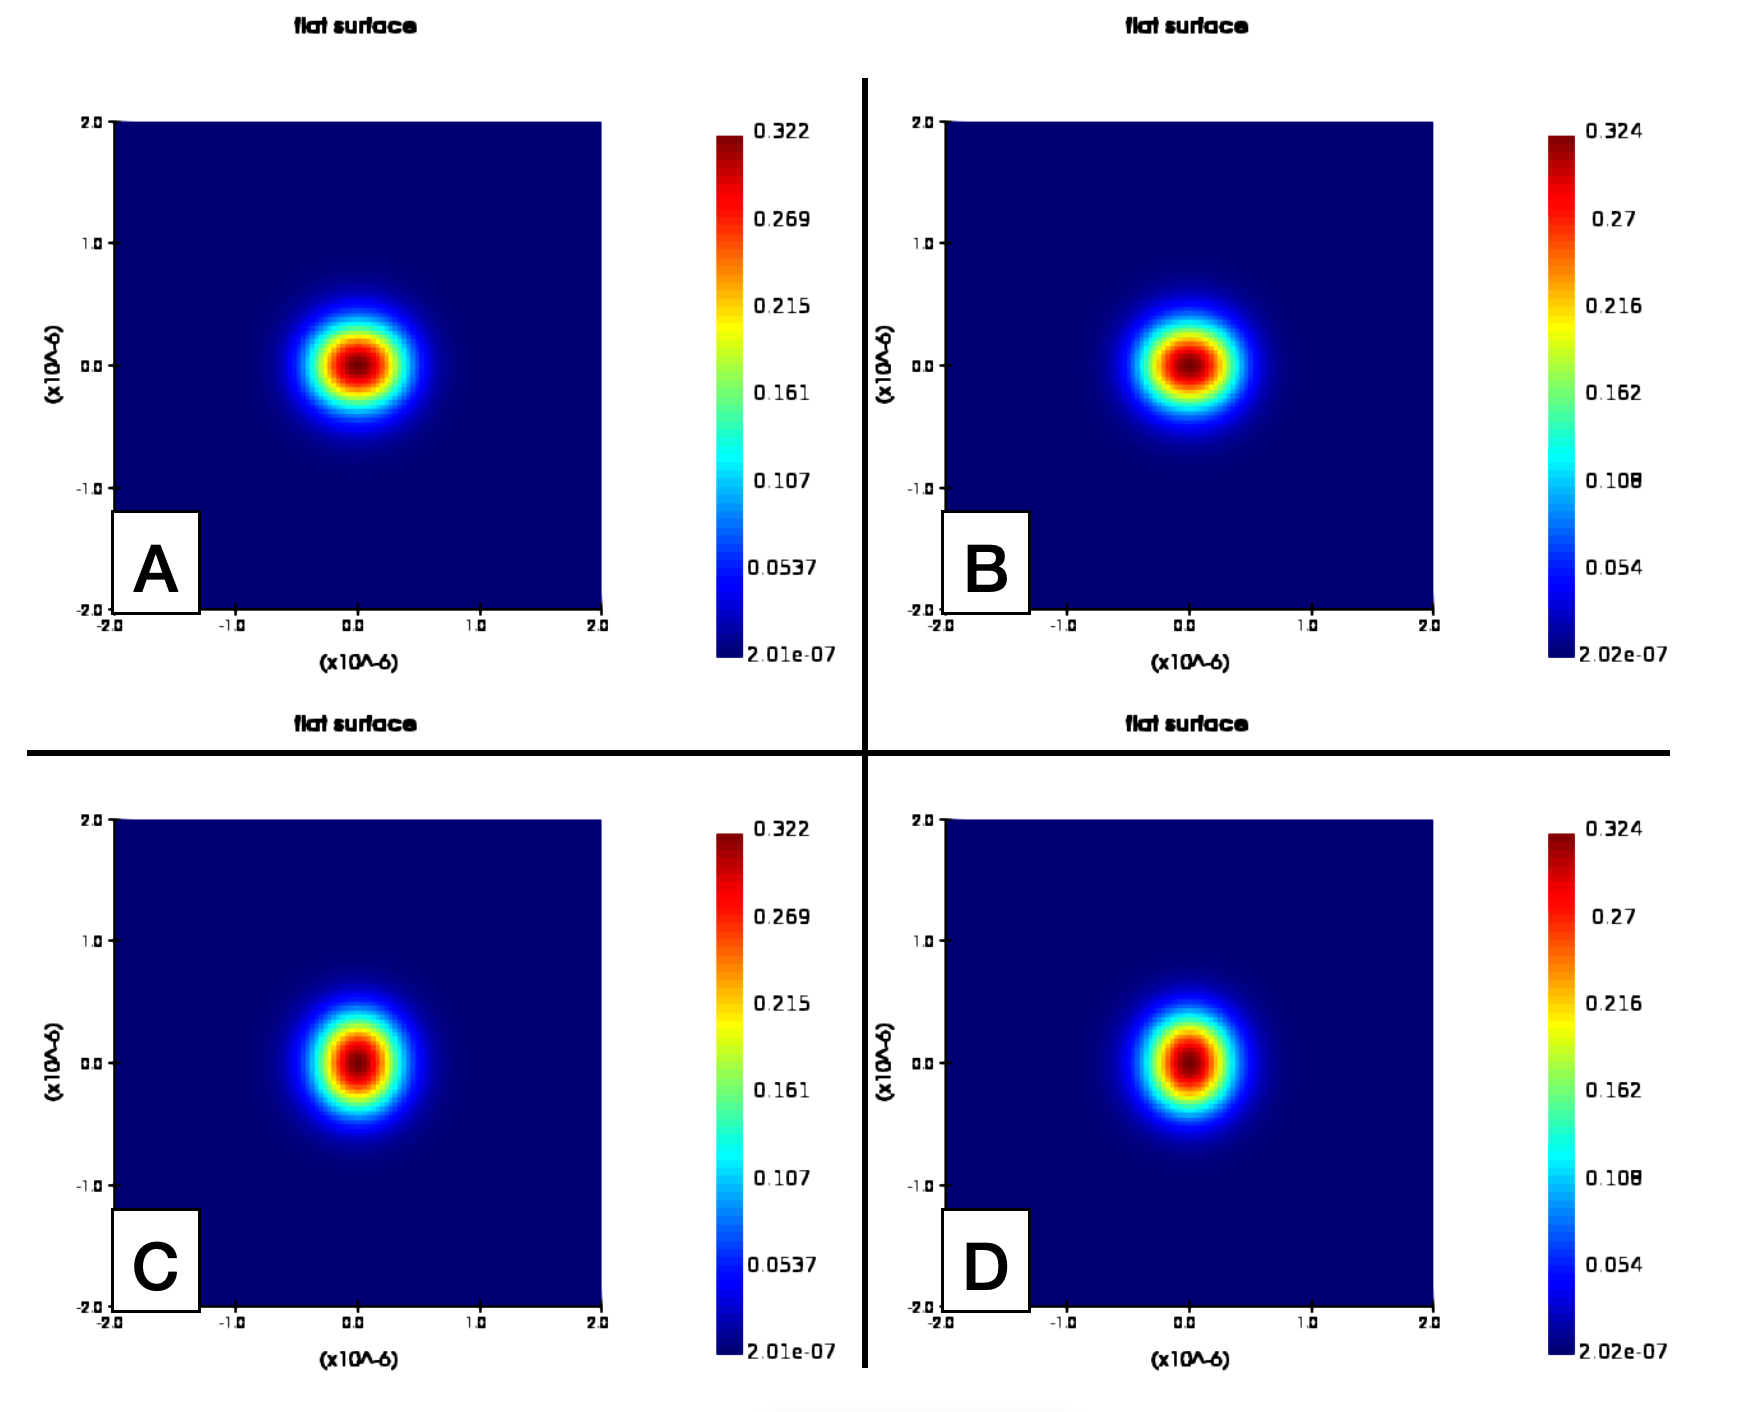
\includegraphics[width=0.95\textwidth]{2.png}
        \caption{Near field picture for the flat surface. A - $0\deg$ polarization simulation. B - $0\deg$ polarization simulation, with boundary conditions applied. C - $90\deg$ polarization simulation. D - $90\deg$ polarization simulation, with boundary conditions applied.}
\end{figure}
\begin{figure}
        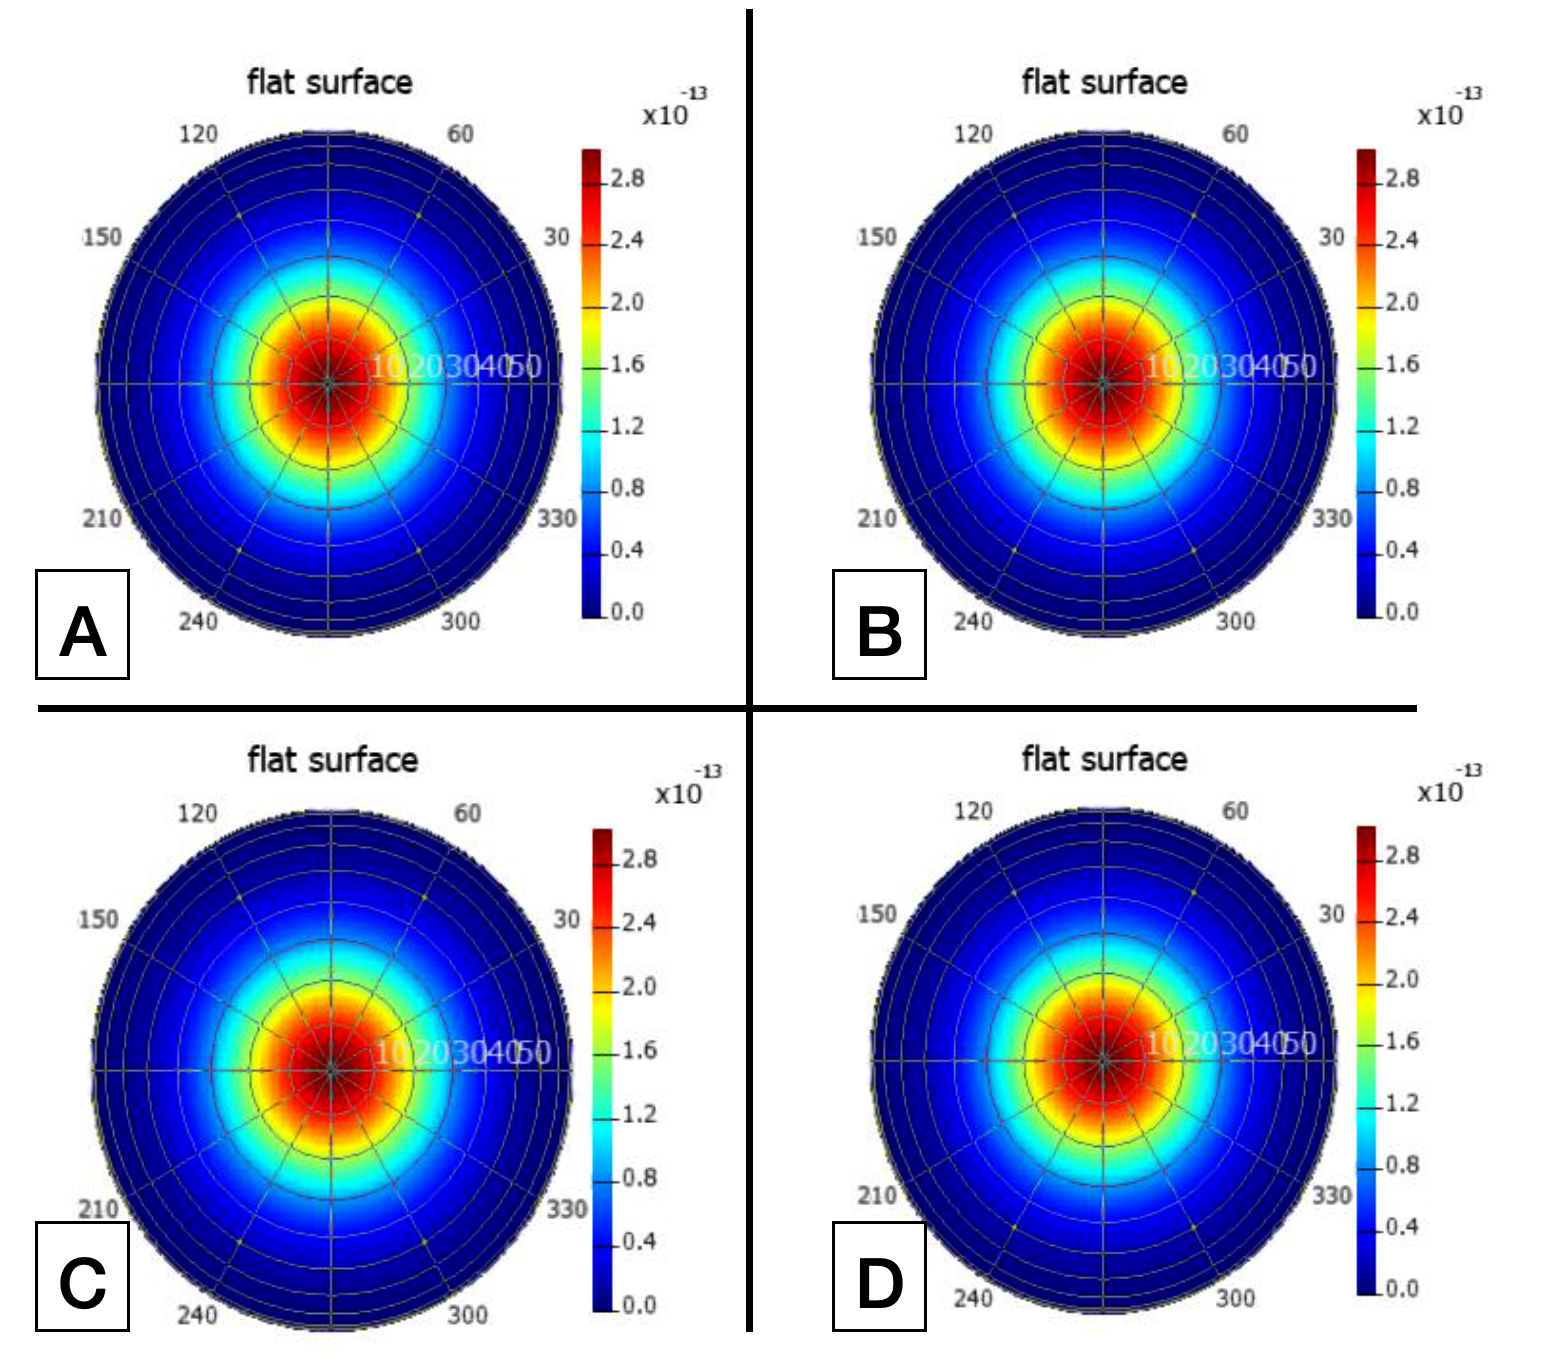
\includegraphics[width=0.95\textwidth]{3.png}
        \caption{Far field polar plot for the flat surface. A - $0\deg$ polarization simulation. B - $0\deg$ polarization simulation, with boundary conditions applied. C - $90\deg$ polarization simulation. D - $90\deg$ polarization simulation, with boundary conditions applied.}
\end{figure}
\begin{figure}
        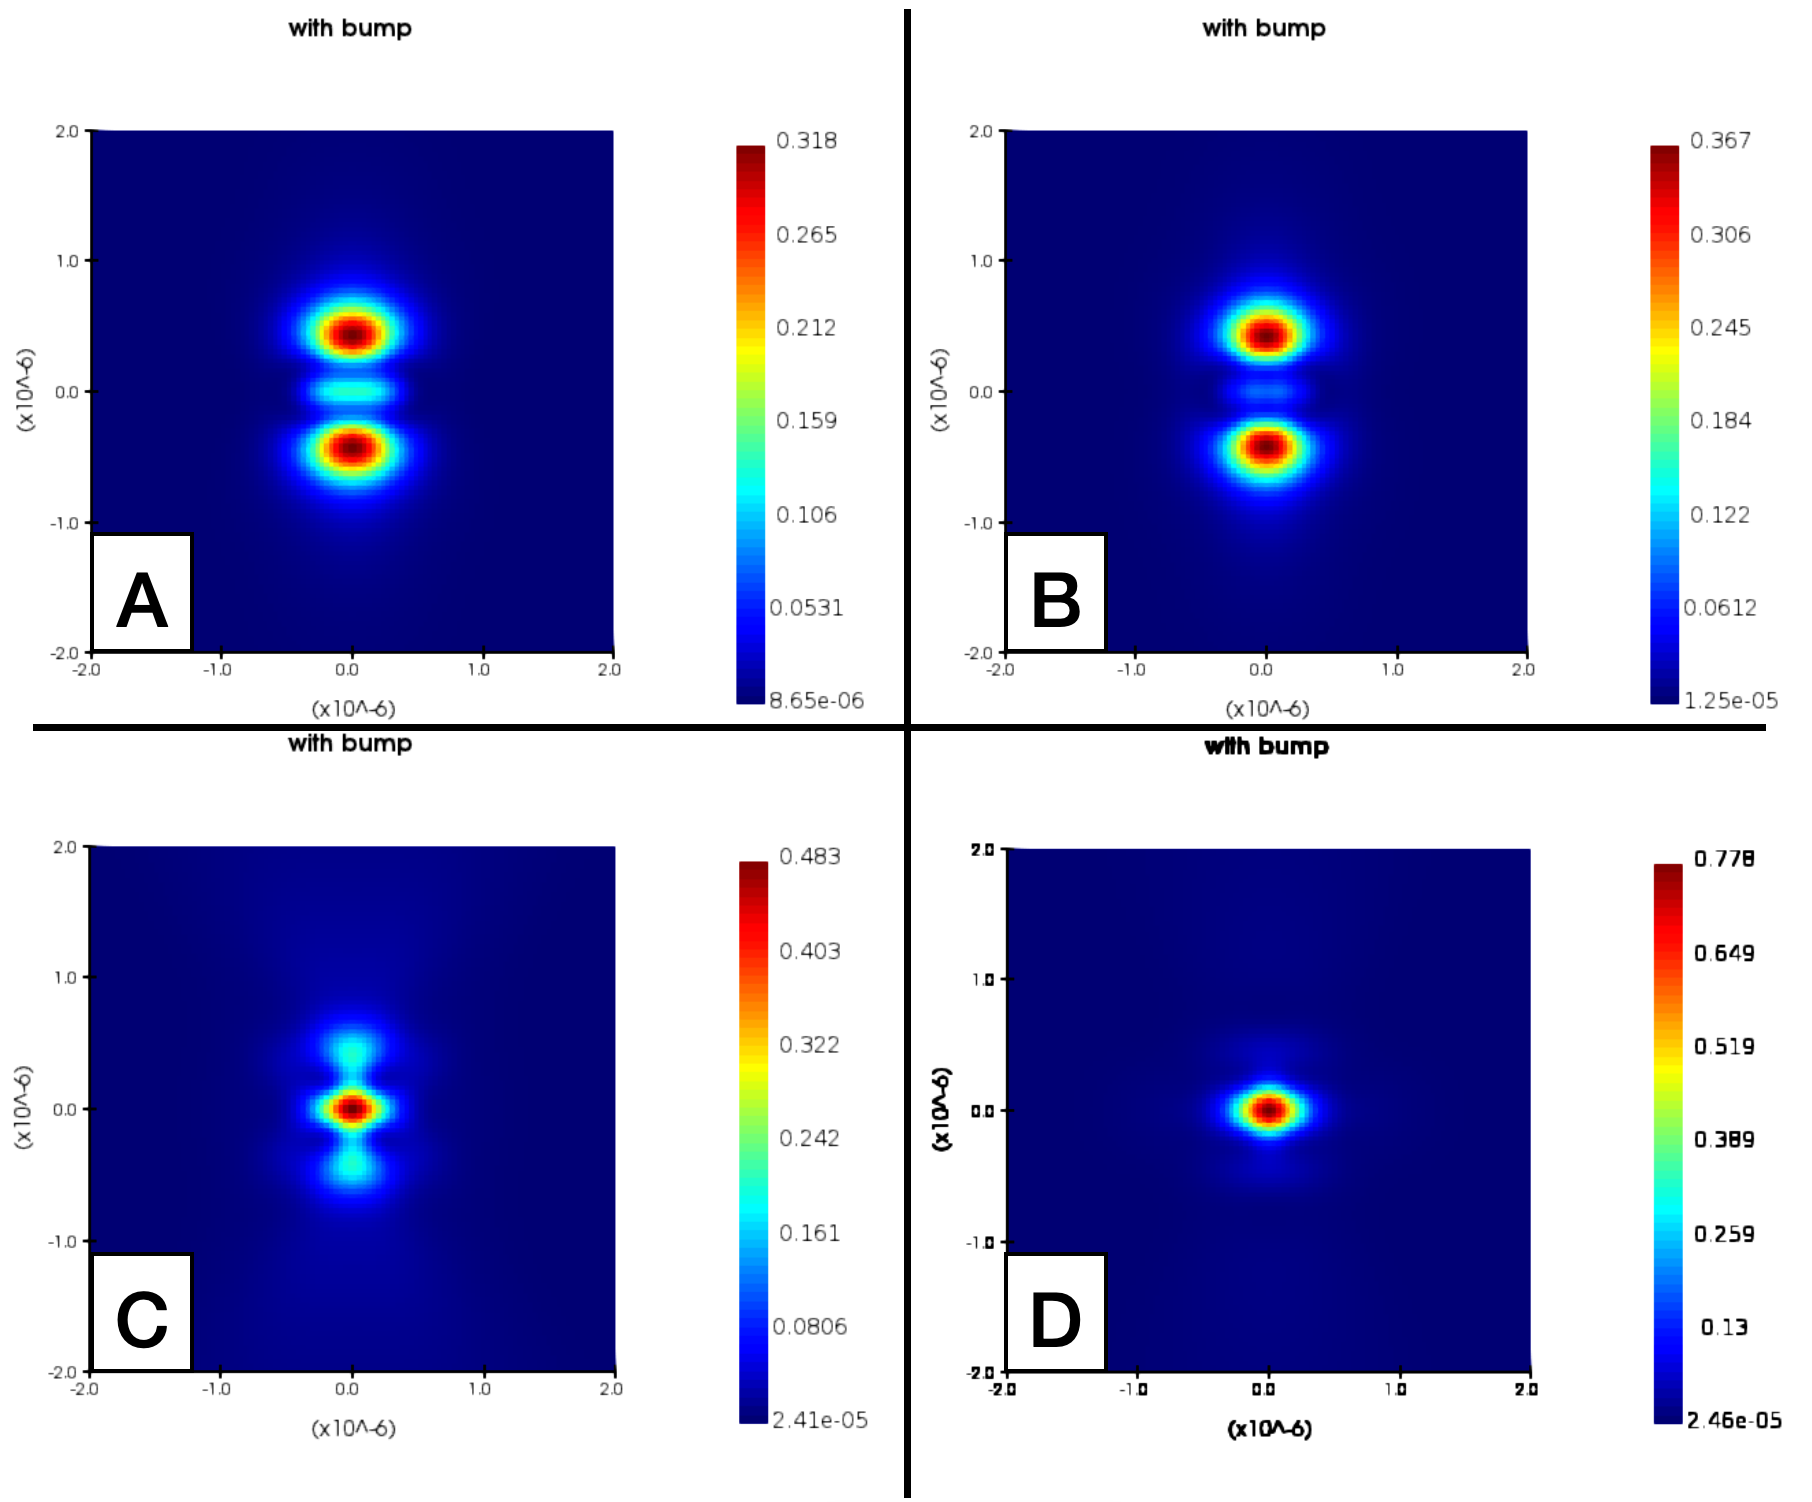
\includegraphics[width=0.95\textwidth]{4.png}
        \caption{Near field picture for the surface with a bump. A - $0\deg$ polarization simulation. B - $0\deg$ polarization simulation, with boundary conditions applied. C - $90\deg$ polarization simulation. D - $90\deg$ polarization simulation, with boundary conditions applied.}
\end{figure}
\begin{figure}
        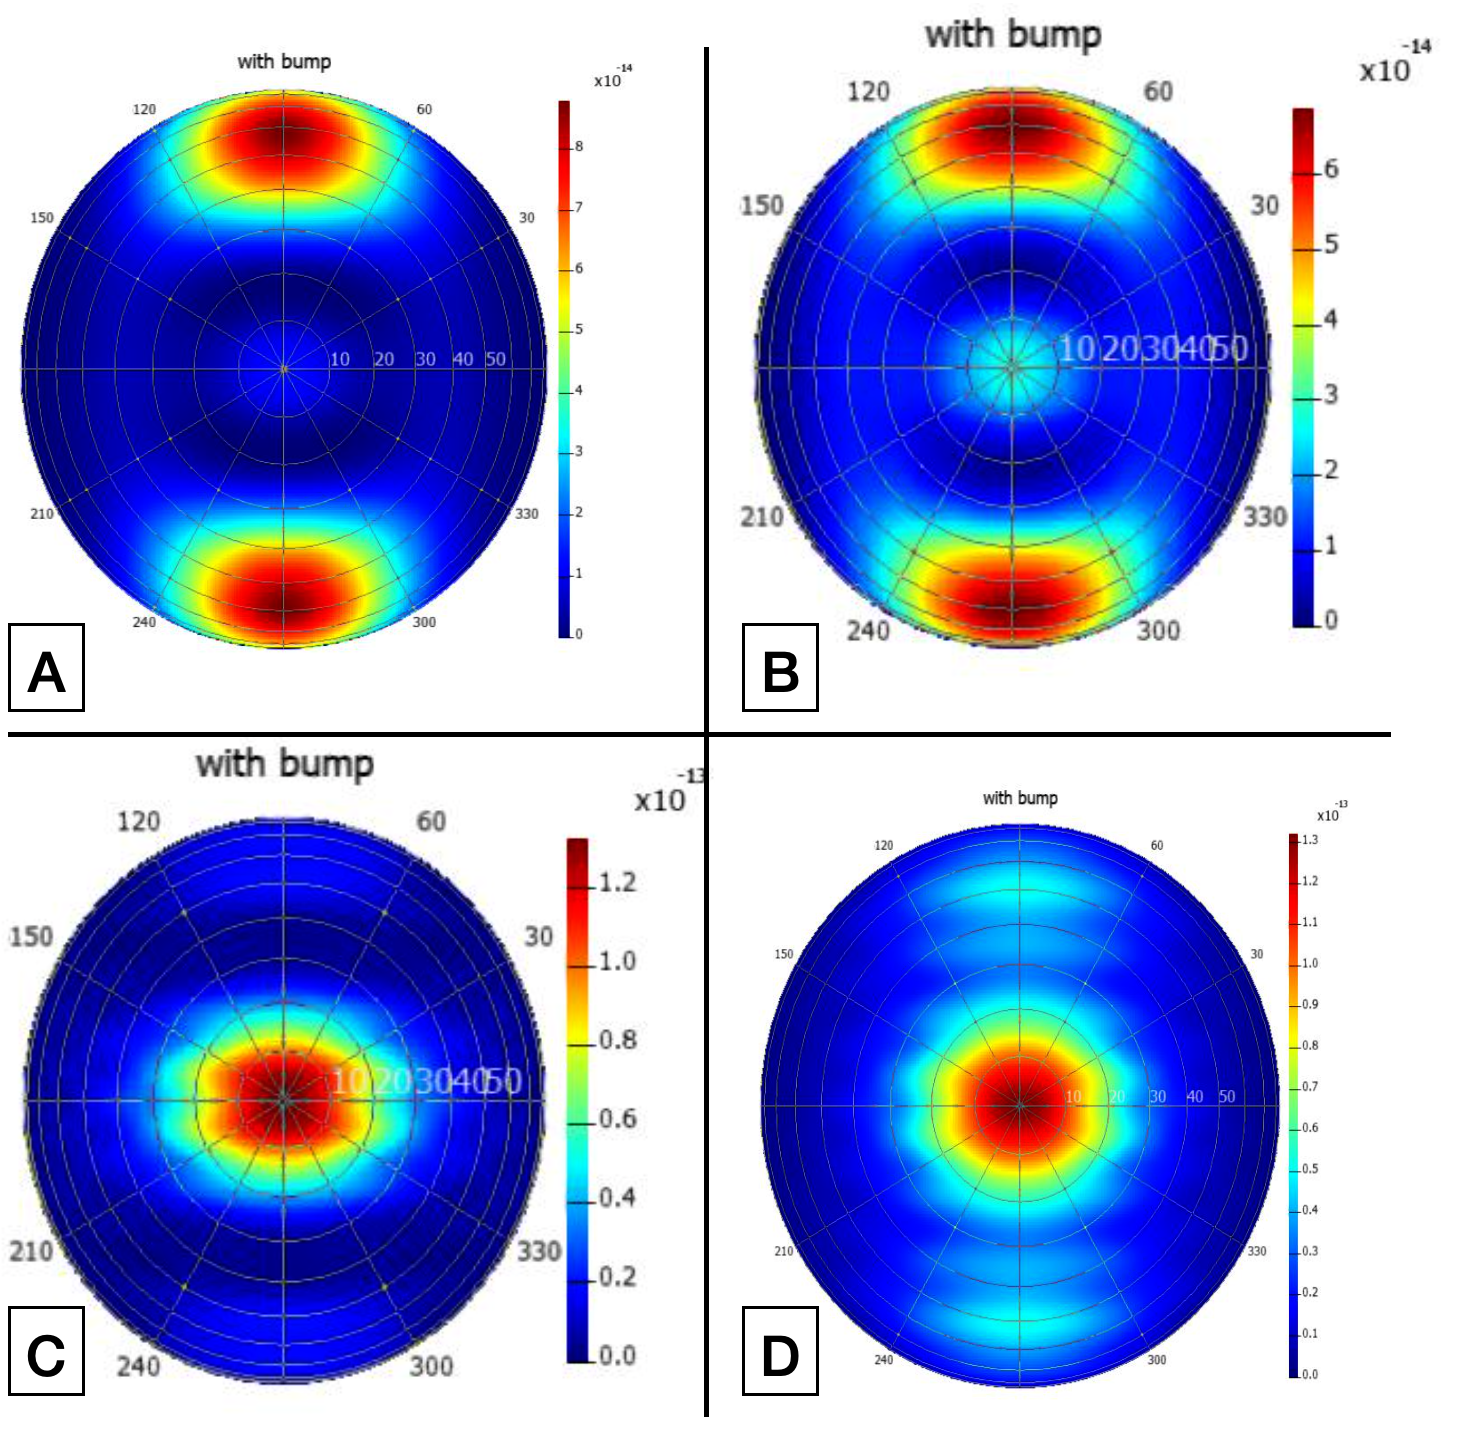
\includegraphics[width=0.95\textwidth]{5.png}
        \caption{Far field polar plot  for the surface with a bump. A - $0\deg$ polarization simulation. B - $0\deg$ polarization simulation, with boundary conditions applied. C - $90\deg$ polarization simulation. D - $90\deg$ polarization simulation, with boundary conditions applied.}
\end{figure}

\begin{figure}
        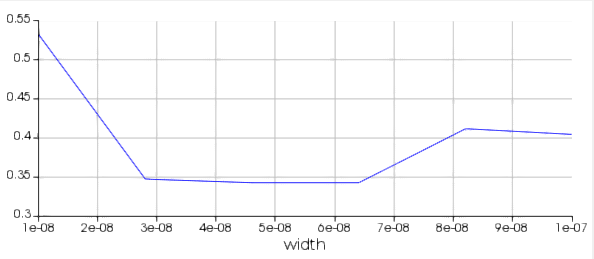
\includegraphics[width=0.95\textwidth]{signal-width_sweep.png}
        \caption{Signal width sweep.}
\end{figure}
\begin{figure}
        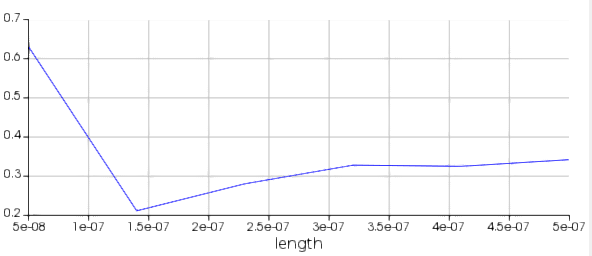
\includegraphics[width=0.95\textwidth]{signal-length_sweep.png}
        \caption{Signal length sweep.}
\end{figure}

\begin{figure}
        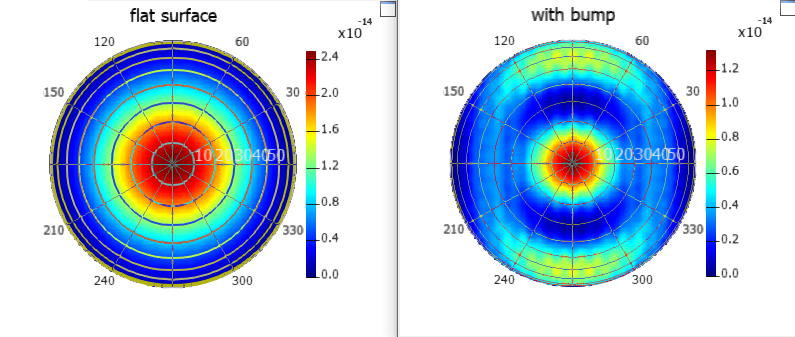
\includegraphics[width=0.95\textwidth]{smaller_farfield.png}
        \caption{Far-field with and without bump for Blu-ray.}
\end{figure}
\begin{figure}
        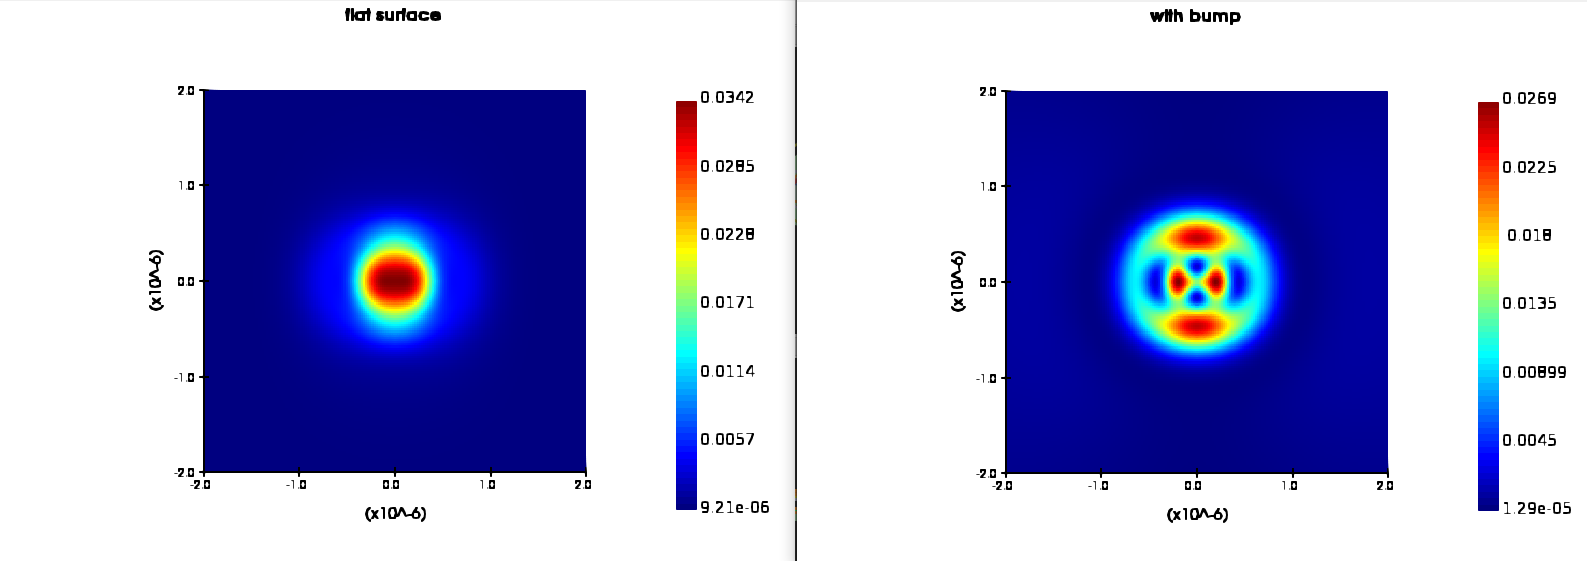
\includegraphics[width=0.95\textwidth]{smaller_nearfield.png}
        \caption{Near-field with and without bump for Blu-ray.}
\end{figure}
\end{document}
